\documentclass[12pt,a4paper]{article}
\usepackage{physics}
\usepackage{amssymb}
\usepackage{subcaption}
\usepackage{colortbl}
\newcommand{\activity}{Activity 4 -- Rendering Color}
\input{spp.dat}

%  Editorial staff will uncomment the next line
% \providecommand{\artnum}[0]{XX-XX}
% \renewcommand{\articlenum}[0]{SPP-\the\year-\artnum-}

\begin{document}

\title{\TitleFont \activity}
\author[ ]{\textbf{Kenneth V. Domingo} \\
2015--03116 \\
App Physics 187, 1\textsuperscript{st} Semester, A.Y. 2019--20}
\affil[ ]{\corremail{kvdomingo@up.edu.ph} }

\maketitle
\thispagestyle{titlestyle}

\section*{Results and Discussion}
\setcounter{section}{1}

For this activity, I used the light source emittance data and leaf reflectance data that our group obtained from the previous activities. Our reference light source is a 20W LED with a CCT of 6500K. All images were taken with a Nikon D3400 with the white balance set to daylight. Since I could not find any spectral information about my camera online, I got the spectral sensitivity data for the Nikon D70 from \cite{naelab} instead.

\subsection{Pre-processing}
Since the number of data points of the spectra were not equal, I had to interpolate some data points so that they were all equalized to the spectra with the most number of data points. Since all the intensities were relative, I then normalized all the spectra to 1.

\subsection{Color rendering}
The color of the leaf was rendered digitally using the light emittance spectrum $M$, the leaf reflectance spectrum $R$, and the camera spectral sensitivity $S$. The RGB values were generated according to \cite{soriano}

\begin{eqnarray}
	Q_i = \int_{\mathrm{visible}} M(\lambda) R(\lambda) S_i(\lambda) \dd{\lambda} \label{eq:sensor-model-integrate} \\
	DN_i = \frac{\sum M(\lambda) R(\lambda) S_i(\lambda)}{\sum M(\lambda) S_i(\lambda)} \label{eq:sensor-model-sum}
\end{eqnarray}

\noindent
The actual and generated colors are shown in Fig. \ref{fig:render}. We can see that the reconstructed color already captures the general color of the leaf.

\begin{figure}[htb]
	\centering
	\begin{subfigure}[h!]{0.49\textwidth}
		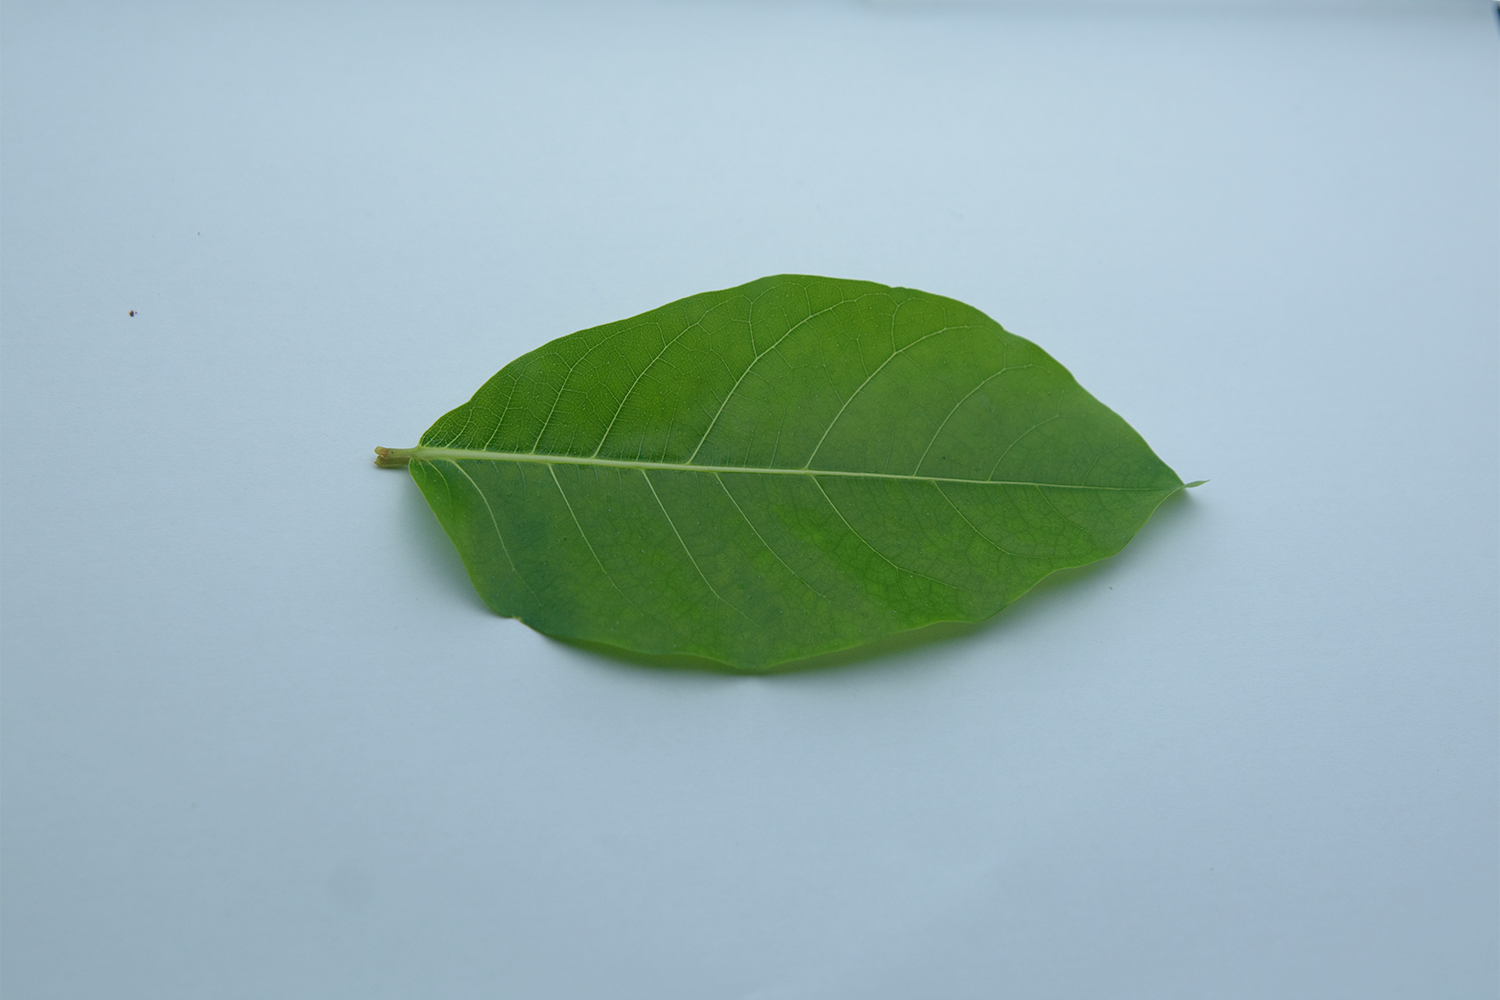
\includegraphics[width=\textwidth]{leaf1.png}
		\caption{actual}
		\label{fig:leaf-actual}
	\end{subfigure}
	\begin{subfigure}[h!]{0.33\textwidth}
		
\includegraphics[width=\textwidth]{render.png}
		\caption{rendered}
		\label{fig:leaf-render}
	\end{subfigure}
	\caption{Actual and rendered colors of a leaf.}
	\label{fig:render}
\end{figure}

To further verify the calculations, we attempt to reconstruct the colors from a Macbeth Color Checker provided by \cite{soriano}. The measured reflectances per patch was also provided and all computations proceed as before. However, on the first attempt, the colors looked way off. I realized that I was still using the emittance from the light source that we used in the previous activity, and that was most likely causing the error. On a hunch, I tried to search for the spectral distribution of a standard D65 illuminant. I was able to obtain spectral data from \cite{d65}, and the final rendered colors are shown in Fig. \ref{fig:macbeth}. From these figures, we can see that the rendered colors are generally more saturated than the actual, while the gray patches are much less saturated.

\begin{figure}[htb]
	\centering
	\begin{subfigure}[h!]{0.45\textwidth}
		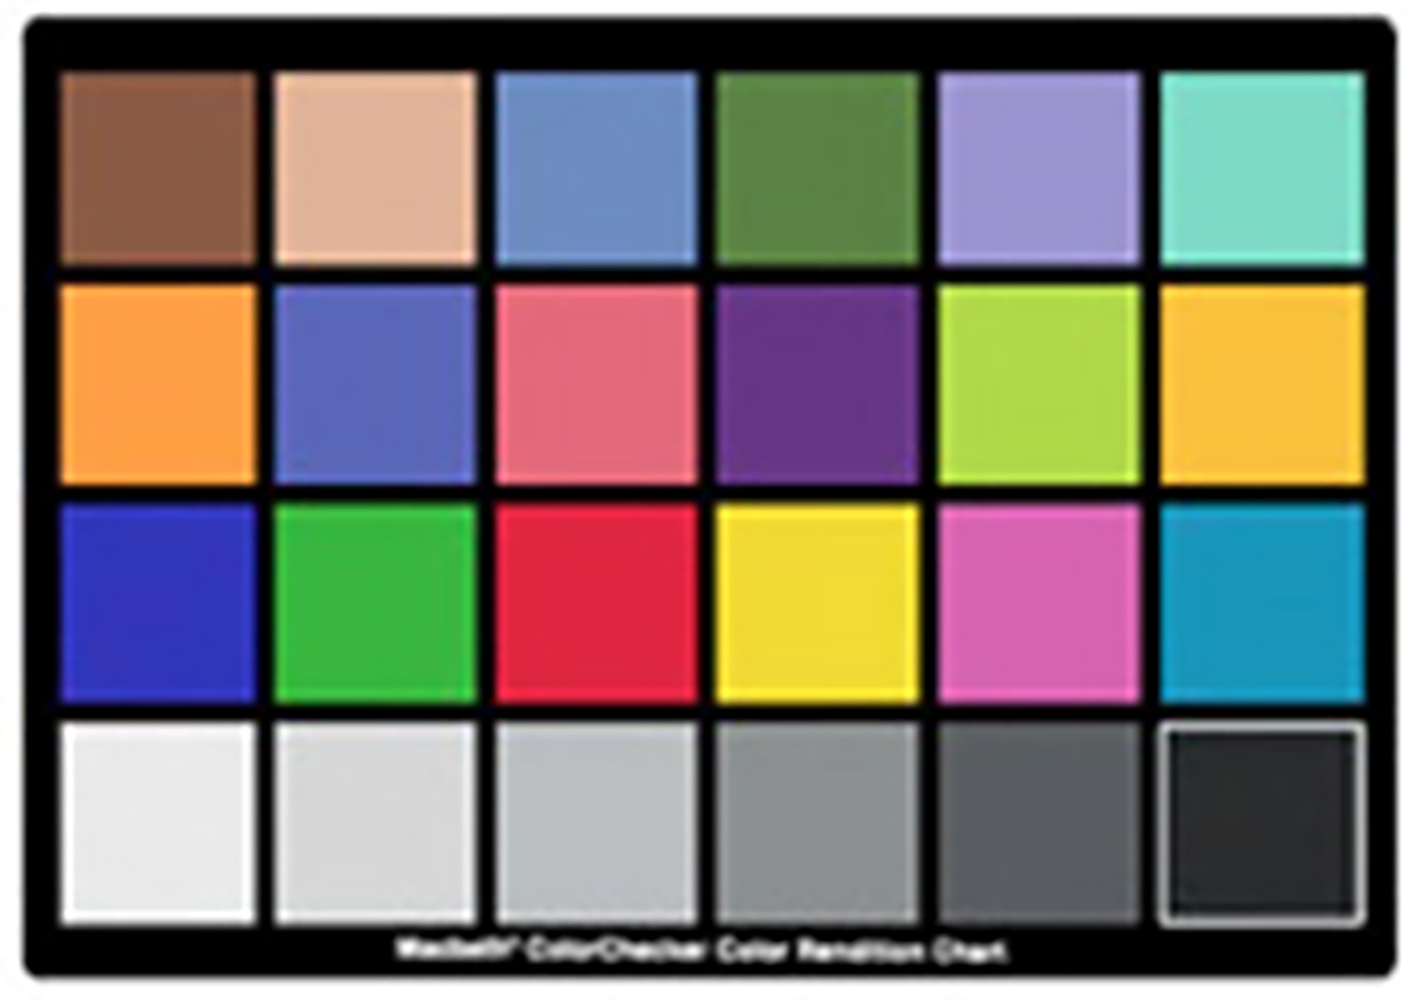
\includegraphics[width=\textwidth]{macbeth.png}
		\caption{actual}
		\label{fig:macbeth-actual}
	\end{subfigure}
	\begin{subfigure}[h!]{0.49\textwidth}
		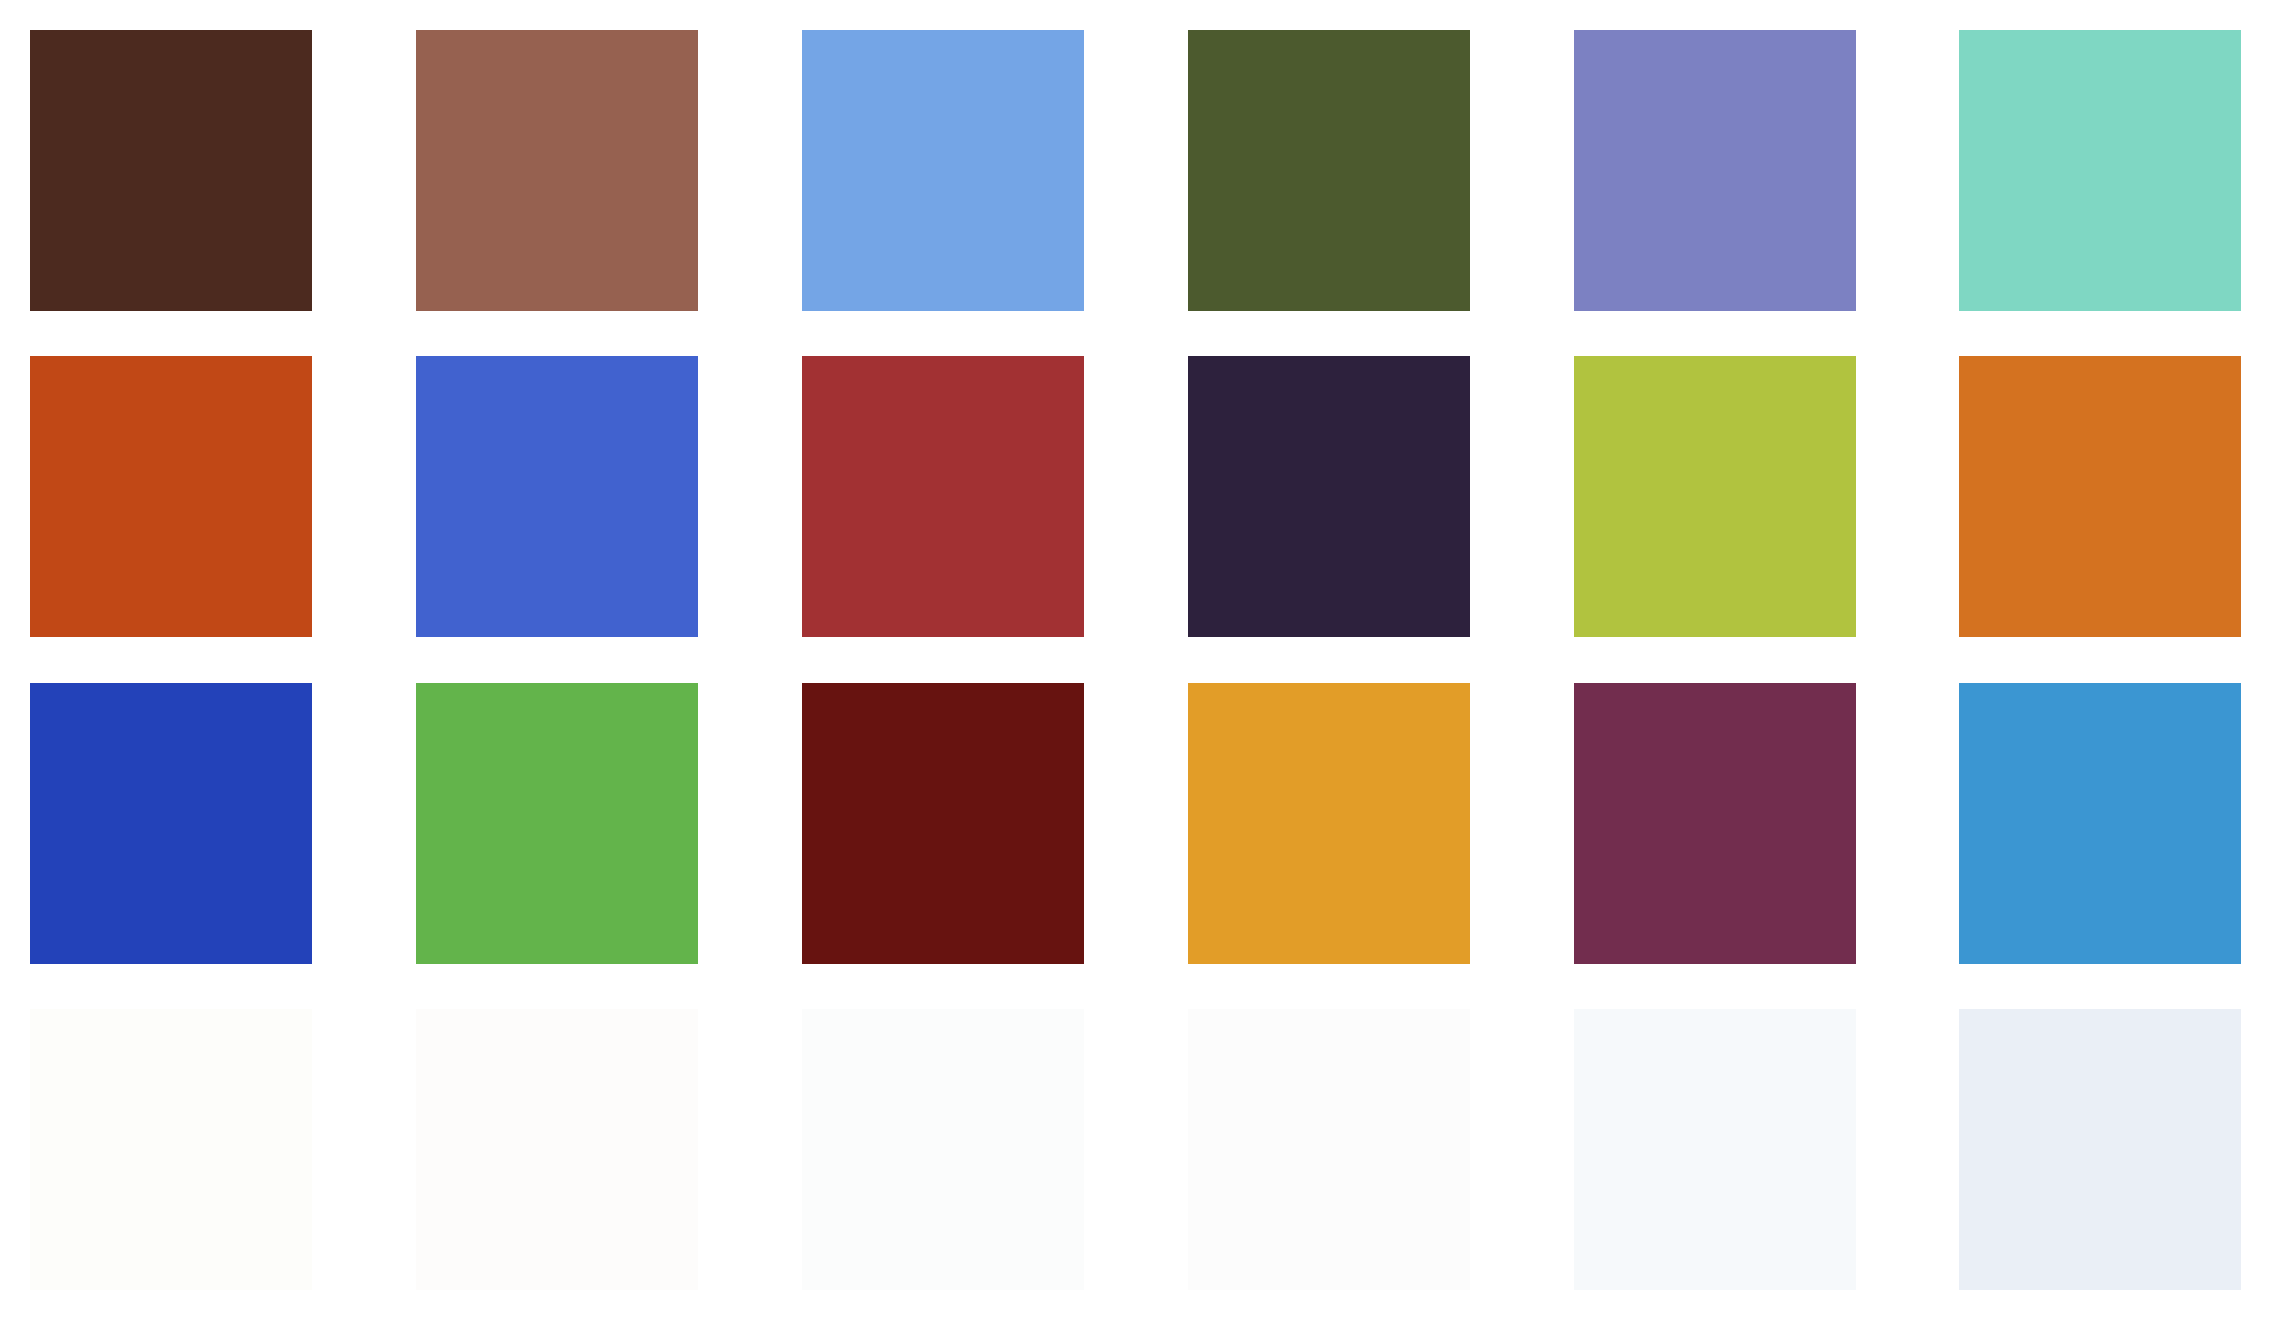
\includegraphics[width=\textwidth]{mac_rendered.png}
		\caption{rendered}
		\label{fig:macbeth-render}
	\end{subfigure}
	\caption{Actual and rendered colors of a Macbeth Color Checker.}
	\label{fig:macbeth}
\end{figure}

\bibliographystyle{spp-bst}
\bibliography{187-Act4}

\end{document}